% Chapter Template

\chapter{Describing cells} % Main chapter title

\label{Chapter6} % Change X to a consecutive number; for referencing this chapter elsewhere, use \ref{ChapterX}


Once cells have been segmented and their fluorescence intensities classified, they are assigned with features that describe human perception of the cells' properties. The interesting properties are summarized in the following section. \\

This step maps \textit{pixel features} to \textit{symbolic features} used to describe the cells. Those symbolic features are learned by \textit{Deep belief network}.


%----------------------------------------------------------------------------------------
%	FEATURES
%----------------------------------------------------------------------------------------

\section{Interesting features}

In \cite{FoggiaBenchmarks2013}, Foggia et al. summarizes the description of interesting properties for each type of cells. Table \ref{tab:Desc} provides a description of every cell type. The problem with such descriptions is that they are quite unstructured and sometimes ubiquitous. For example, when speaking about organelles contained in a cell's body, they refer to dark organelles as \textit{granules} and bright organelles as \textit{speckles}. \\

In order to develop a method that will generate such descriptions automatically, these description should be structured first. Table \ref{tab:Vpata} gives a general description of each pattern in a more structured way. The appearance of patterns varies for the general descriptions depending on the fluorescence intensity of an image. Several important visual patterns were identified. \\

The first property describes the shape of a cell. It can take two possible values - \textit{circular} and \textit{irregular}. The motivation for this feature is the observation that the irregular shape is very characteristic for the cytoplasmatic class, while all other classes have a circular shape. \\

The property \textit{speckles} denotes are there any objects present in the cell or not. \\

Incorporating the knowledge about the mitotic cells found on the same image can be quite useful.Medical literature suggested that the mitotic cells, although there is no general consensus about their importance, might be informative for discriminating between certain patterns. The mitotic cells can appear in four different patterns - \textit{neutral} with no specific characteristics, \textit{bright center},  \textit{bright center} with sparkles or \textit{dark center}. For now, the type of mitotic cell is manually assigned. \\

The following property describes the appearance of organelles in a cell's body, if there are any. This property is very discriminatory towards the nucleolar and the centromere which have bright organelles, speckled which contain dark organelles while others don't have any organelles. \\

The number of organelles is also an informative property. The centromere pattern has significantly larger numbers of organelles contained in a body. The centromene, the nucleolar and the speckled patterns contain relatively small numbers of organelles expressed in the body, while the homogeneous and cytoplasmatic class don't have any organelles. \\

For certain patterns, the texture could be quite informative. Although most of the patterns have a relatively smooth texture, some patterns have some very distinguishing properties. On images with positive fluorescence intensity, the cytoplasmatic class has a characteristic blob. Also, the coarse speckled class has a very specific texture that looks like the \textit{sea surface}. \\

\textbf{Shape classification.} As shape classification is not performed with the Deep belief network, the results are presented here. For this step, the segmentation masks are used and classified with SVM as described is Chapter \ref{Chapter5}. The smallest rectangle that can fit the mask is divided in 6 cells - 2 horizontally and 3 vertically. For each cell, a ratio of the background and a cell pixels is calculated and used as a feature. Those 6 features were then used to train the SVM. The results are summarized in table \ref{tab:ShpInt}. The 10-fold cross validation is used to validate method. The achieved accuracy is 98.68 \%. The information about the \textit{irregular} shape is very informative about the cytoplasmatic pattern,it is important that both precision and recall are high for the class. In this case, that condition is satistied, have the precision equal to 93.57 \% and recall 95.32 \%.  \\



\begin{table}
	\begin{center}
	\caption{Description of cell types}
	\label{tab:Desc}
	\begin{tabular}{|m{2.3cm}|m{2.1cm}|m{8cm}|}
		\hline
		\textbf{pattern type} & \textbf{example} & \textbf{description} \\
		\hline
		centromere & 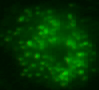
\includegraphics[width=2cm]{Figures/describing/centromere} & characterized by several 			discrete speckles ($ \approx 40-60$) distributed throughout the interphase nuclei and 		characteristically found in the condensed nuclear chromatin during mitosis as a bar of closely associated speckles. \\ \hline
		nucleolar & \vspace{5pt} 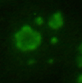
\includegraphics[width=2cm]{Figures/describing/nucleolar} & characterized by clustered 			large granules in the nucleoli of interphase cells which tend towards homogeneity, with less than six granules per cell. \\ \hline
		homogeneous & \vspace{5pt} 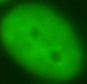
\includegraphics[width=2cm]{Figures/describing/homogeneous} & characterized by a 	diffuse staining of the interphase nuclei and staining of the chromatin of mitotic cells. \\ \hline
		
		fine speckled & \vspace{5pt} 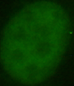
\includegraphics[width=2cm]{Figures/describing/fine_speckled} & characterized by a 			fine granular nuclear staining of the interphase cell nuclei \\ \hline
		
		coarse speckled & \vspace{5pt} 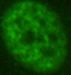
\includegraphics[width=2cm]{Figures/describing/coarse_speckled} & characterized by a coarse granular nuclear staining of the interphase cell nuclei \\ \hline
		
		cytoplasmatic & \vspace{5pt} 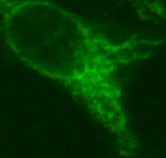
\includegraphics[width=2cm]{Figures/describing/cytoplasmatic} & characterized by a specific shape and large granule \\ \hline
	\end{tabular}
	\end{center}
\end{table}

\begin{table}
	\caption{Identified visual patterns - positive intensity}
	\label{tab:Vpata}
	\small
	\begin{tabular}{|m{2.2cm}|m{1.4cm}|m{1.5cm}|m{1.5cm}|m{1.4cm}|m{1.6cm}|m{1.4cm}|}
		\hline
		\textbf{pattern type} & \textbf{shape} & \textbf{mitotic cell} & \textbf{organelle type} & \textbf{organelle count} & \textbf{texture} & \textbf{speckles} \\ \hline
		centromere & circular & bright with sparkles & bright on dark & lots & sparkly  & yes \\ \hline
		nucleolar & circular & neutral & bright on dark & few & smooth & yes \\ \hline
		cytoplasmatic & irregular & dark spot & dark on bright & none & blob / smooth  & no \\ \hline
		homogeneous & circular & bright & neutral & none & smooth & no \\ \hline
		fine speckled & circular & neutral / dark & neutral / dark & none & smooth & no \\ \hline
		coarse speckled & circular & dark & dark on bright & few & rough & yes \\ \hline
	\end{tabular}
	\normalsize
\end{table}

\begin{table}
	\centering
	\caption{Performance of shape classification}
	\label{tab:ShpInt}
	\begin{tabular}{c c| c c}
				 & & \multicolumn{2}{c}{True} \\
			     & & \textbf{circ} & \textbf{irr} \\
			    \hline
			    \multirow{2}{*}{\rotatebox[origin=c]{90}{Pred}} & \textbf{circ} & \cellcolor{gray}99.62 \% & 6.43 \% \\
			    & \textbf{irr} & 0.38 \% & \cellcolor{gray}93.57 \%
			\end{tabular} 
\end{table}



%--------------------------------------------%
%                                            %
%             DEEP LEARNING                  %
%                                            %
%--------------------------------------------% 

\section{Deep learning}

Deep learning is a relatively new approach in machine learning which is often referred  as \textit{Representation learning}. It is built upon \textit{Artificial neural networks} and imitates the human brain in representing  data. The motivation for learning representation is quite clear -- the form in which data is represented is important. The success of our classifier depends on the quality of data used for training. \\

The key concept used in Deep learning is a \textit{hierarchical representation of data}. Deep learning aims at learning feature hierarchies with features from higher levels of the hierarchies formed by composing lower level features. Automatically learning features at multiple levels of abstraction allows a system to learn complex functions representing the data, without depending completely on human-crafted features. That is particularly important because humans often do not know how to express higher-level abstraction in terms of raw sensory input. The ability to automatically learn powerful features will become increasingly important as the amount of data and range of applications of machine learning methods continues to grow. \\

Consider a computer vision framework, for example. Raw input corresponds to raw pixels of an image. The idea of Deep learning is to gradually \textit{abstract} the pixels to higher level features. Raw pixels are further combined to form edges, edges are then abstracted to specific forms and so on. The focus of deep architecture learning is to automatically discover such abstractions, from the lowest level features to the highest level concepts. Ideally, we would like learning algorithms that enable this discovery with as little human effort as possible. \\

Depth of architecture refers to the number of levels of composition of non-linear operations in the function learned. Most of current machine learning algorithms correspond to \textit{shallow architectures} while the brain is organized in \textit{deep architectures}, with multiple levels of abstraction. \\

Another important thing to notice is that the information is \textit{distributed}: in the brain analogy, the information is not localized in a particular neuron but distributed across many. Each level of abstraction found in the brain consists of the \textit{activation} (neural excitation) of a small subset of a large number of features that are, in general, not mutually exclusive. In addition to being distributed, it appears that the brain uses a representation that is \textit{sparse}: only around 1-4\% of the neurons are active together at a given time.

%--------------------------------------------%
%                                            %
%           DEEP BELIEF NETWORKS             %
%                                            %
%--------------------------------------------%

\section{Deep belief networks}

The Deep belief network is a specific instance of the deep learning approach. It can be seen as a multi-layer generative model where each layer consists of multiple nodes, similar to a neural network. The first layer, often referred as the \textit{visible layer}, represents the raw input data, while every higher-level layer is referred to as the \textit{hidden layer}. The main difference between deep belief networks and neural networks is an \textit{unsupervised} pre-training phase of a deep belief network. \\

To train the network in unsupervised way, the network is represented using the \textit{Restricted Boltzmann machines}.





\subsection{Restricted Boltzmann Machines}

Boltzmann machines are an instance of \textit{energy-based} models, in which  scalar energy is associated  to each configuration of variables. Learning in such settings corresponds to modifying the energy function so that it reflects certain properties -- support desired ones and discourage. The  Boltzmann machines are trained by maximizing the probability of data:

\begin{equation}
	 \arg\max_{W}\prod_{v \in V}P(\mathbf{v})
\end{equation}	
	
%	$$ \arg\max_{W}\prod_{v \in V}P(\mathbf{v}) $$
	
where $\mathbf{v}$ represent a raw data. Energy-based probabilistic models define  probability distribution over a variable through an energy function

\begin{equation}
	P(\mathbf{x}) = \frac{e^{-\mathtt{Energy}(\mathbf{x})}}{Z}.
\end{equation}

The normalization factor $Z$ is called the \textit{partitioning function} by analogy with physical systems
\begin{equation}
	Z = \sum_{\mathbf{x}}e^{-\mathtt{Energy}(\mathbf{x})}
\end{equation}
 with a sum running over the input space. The energy function is usually formulated as a sum of term $f_i$
 
 \begin{equation}
 	\mathtt{Energy}(\mathbf{x}) = \sum_i f_i(\mathbf{x}),
 \end{equation}
 
 where each $f_i$ evaluates some properties of an input vector $\mathbf{x}$. \\
 
 In the case of hidden variables, probability is expressed as 
 
 \begin{equation}
	P(\mathbf{x}, \mathbf{h}) = \frac{e^{-\mathtt{Energy}(\mathbf{x}, \mathbf{h})}}{Z},
\end{equation}
 
 where probability of the observed part can be calculated by marginalization
 
 \begin{equation}
	P(\mathbf{x}) = \sum_{\mathbf{h}}\frac{e^{-\mathtt{Energy}(\mathbf{x}, \mathbf{h})}}{Z}.
\end{equation}

Conditional probability distributions can be efficiently represented in the energy-based framework

\begin{equation}
	P(y| \mathbf{x}) = \frac{e^{-\mathtt{Energy}(\mathbf{x},y)}}{\sum_y e^{-\mathtt{Energy}(\mathbf{x},y)}}.
\end{equation}

The Boltzmann machine defines the energy functional as a second-order polynomial

\begin{equation}
	\mathtt{Energy}(\mathbf{x}, \mathbf{h}) = -\mathbf{b}^T\mathbf{x} - \mathbf{c}^T\mathbf{h} - \mathbf{h}^T\mathbf{W}\mathbf{x} - \mathbf{x}^T\mathbf{U}\mathbf{x} - \mathbf{h}^T\mathbf{V}\mathbf{h}
	\label{eq:BoltzmannEnergy}
\end{equation}

where $\mathbf{x}$ represents raw data, $\mathbf{h}$ response of hidden units, $\mathbf{b}_i \text{ and } \mathbf{c}_i$ are the offsets associated with a single element from $\mathbf{x}$ or $\mathbf{h}$ and $W_{ij}, U_{ij} \text{ and } V_{ij}$ are weights associated with each pair of units. \\

The \textit{restriction} in the Restricted Boltzmann machines comes from connections within a layer. In the Restricted Boltzmann machine there are no connections within a layer, only connections between successive layers. The output of each layer serves as the input for the successive layer.  This restriction simplifies the equation \ref{eq:BoltzmannEnergy} and eliminates the factors $U$ and $V$. The equation \ref{eq:BoltzmannEnergy} is now

\begin{equation}
	\mathtt{Energy}(\mathbf{x}, \mathbf{h}) = -\mathbf{b}^T\mathbf{x} - \mathbf{c}^T\mathbf{h} - \mathbf{h}^T\mathbf{W}\mathbf{x} 
	\label{eq:RestBoltzmannEnergy}
\end{equation}

and has a property that shares it's parameterization with individual layers of a Deep belief network, which makes them perfect building blocks. The restriction is illustrated in figure \ref{img:RestBoltzMach}. Another advantage of the restriction is that it makes calculations of $P(\mathbf{x} | \mathbf{h}) \text{ and } P(\mathbf{h} | \mathbf{x})$ tractable because they factorize.

\begin{figure}
	\begin{center}
		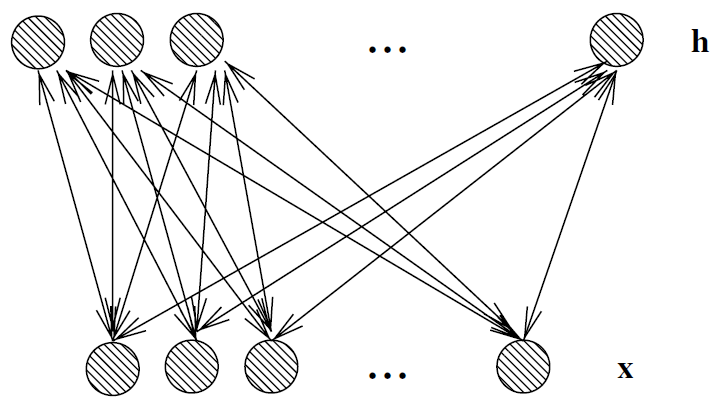
\includegraphics[scale=0.5]{Figures/describing/restricted_boltzmann_machines}
	\end{center}
	\caption{An illustration of the Restricted Boltzmann machines (from \cite{Bengio2009})}
	\label{img:RestBoltzMach}
\end{figure}


\subsection{Training the Restricted Boltzmann machines}

Training the Restricted Boltzmann machine is usually done by gradient descent. It turns out that the standard gradient of the log-likelihood, although in very simple form, is very hard to estimate. The derivative of the log-likelihood parameterized with the weights $\mathbf{w}$ equals

\begin{align}
		\frac{\partial p(\mathbf{x})}{\partial \mathbf{w}} & = \sum_n \mathtt{log} \left [ \frac{1}{Z} e ^{-\mathtt{Energy}(\mathbf{x})}  \right ] \\
		& = N \left [ \left \langle \frac{\partial \mathtt{Energy}(\mathbf{x})}{\partial \mathbf{w}}  \right \rangle_{P(\mathbf{x})} - \left \langle \frac{\partial \mathtt{Energy}(\mathbf{x})}{\partial \mathbf{w}} \right \rangle_n  \right ] \\
		& = \left \langle \mathbf{x}\mathbf{h} \right \rangle_{data} - \left \langle \mathbf{x}\mathbf{h} \right \rangle_{model}
\end{align}

where $\langle \rangle$ marks the expectation under the distribution specified with the subscript. The obtained result lead to a very simple rule for updating weights

\begin{equation}
	\Delta w_{ij} \propto \epsilon \left (  \left \langle x_ih_i   \right \rangle_{data} - \left \langle x_ih_i   \right \rangle_{model}   \right ).
\end{equation}

Estimating $ \langle x_ih_j \rangle_{data}$ is relatively simple as there are no connections between hidden units in a RBM. Given random input data $\mathbf{x}$ the binary state $h_j$ of each hidden unit is set to 1 with probability

\begin{equation}
	p(h_j | \mathbf{x}) = \sigma \left ( b_j + \sum_i x_iw_{ij} \right )
	\label{eq:CDhid}
\end{equation}
where $\sigma$ stands for sigmoid function. $x_ih_j$ is then an unbiased sample. Because there are no connections between visible units in a RBM, it is also easy to get an unbiased sample of the state of a visible unit, given a hidden vector

\begin{equation}
	p(x_i=1 | \mathbf{h}) = \sigma \left ( a_i + \sum_jh_jw_{ij} \right ).
	\label{eq:CDvis}
\end{equation}

Getting an unbiased sample of $ \langle x_ih_j \rangle_{model}$ is much more difficult. An efficient method for estimating that distribution is given in \cite{Hinton2002}. This method starts by assigning training data to visible layer units. Then, the states of the hidden units are evaluated using equation \ref{eq:CDhid}. Once the states for the hidden units have been chosen, the input data is \textit{reconstructed} by setting each $x_i$ to 1 with probability given by equation \ref{eq:CDvis}. The change in weights is then given by 

\begin{equation}
	\Delta w_{ij} = \epsilon \left (  \left \langle x_ih_i   \right \rangle_{data} - \left \langle x_ih_i   \right \rangle_{model}   \right ).
\end{equation}

The method is summarized in Algorithm \ref{alg:RBM}. This assignment could be repeated several times to obtain a better approximation, but just one assignment works surprisingly well. The network is trained the same way layer by layer. \\

Although this approach works very well in practice, it is actually a quite crude approximation of  log-probability. It is more close to an approximation of the \textit{Contrastive Divergence} - the difference between two Kullback-Lieber divergences. \\

\subsubsection{Real valued units}

So far, it has been assumed that all units are binary. That has been done for the sake of simplicity. Binary case is easily generalized to real valued units. The main change is the adjustment of the energy term. For the real valued visible units, Gaussian visible units are a popular choice

\begin{equation}
	\mathtt{Energy}_{G1}(\mathbf{x}, \mathbf{h}) = \sum_{i \in \text{visible}}\frac{(v_i - a_i)^2}{2\sigma_i^2} - \sum_{j \in \text{hidden}} b_jh_j - \sum_{i,j}\frac{v_i}{\sigma_i}h_iw_j
\end{equation}

where $\sigma_i$ is the standard deviation of the Gaussian noise for visible unit $i$. For real valued units in hidden layers, the energy functional looks like

\begin{equation}
	\mathtt{Energy}_{G2}(\mathbf{x}, \mathbf{h}) = \sum_{i \in \text{visible}}\frac{(v_i - a_i)^2}{2\sigma_i^2} - \sum_{j \in \text{hidden}} \frac{(h_j - b_j)^2}{2\sigma_j^2} - \sum_{i,j}\frac{v_i}{\sigma_i}\frac{h_j}{\sigma_j}w_j.
\end{equation}




\begin{algorithm}
	\caption{Training RBM}
	\label{alg:RBM}
	\begin{algorithmic}[1]
		\Function{trainRBM}{$\mathbf{x_1}, \epsilon, W, \mathbf{b}, \mathbf{c}$}
		\Repeat
			\For{all hidden units $i$}
				\State compute $p(h_{1i}=1|\mathbf{x}_1) = \sigma \left ( c_i + \sum_jW_{ij}x_{1j}  \right )$
				\State sample $h_{1i} \in \{ 0,1 \}$ for $p(h_i|\mathbf{x}_!)$
			\EndFor
			
			\For{all visible units $j$}
				\State compute $p(x_{2j}|\mathbf{h}_1) = \sigma \left ( b_j + \sum_iW_{ij}h_{1i} \right )$
				\State sample $x_{2j} \in \{ 0,1 \}$ from $p(x_{2j}|\mathbf{h}_1)$
			\EndFor
			
			\For{all hidden units $i$}
				\State compute $p(h_{2i}=1|\mathbf{x}_2) = \sigma \left ( c_i + \sum_jW_{ij}x_{2j}  \right )$
			\EndFor
			
			\State $W \gets W + \epsilon \left ( \mathbf{h}_1 \mathbf{x}_1^T - p(\mathbf{h}_{2\cdot} = 1|\mathbf{x}_2)\mathbf{x}_2^T\right )$
			\State $\mathbf{b} \gets \mathbf{b} + \epsilon ( \mathbf{x}_1 - \mathbf{x}_2  )$
			\State $\mathbf{c} \gets \mathbf{c} + \epsilon (\mathbf{h}_1 -  p(\mathbf{h}_{2\cdot} = 1|\mathbf{x}_2))$
		\Until{converged}
		\EndFunction
	\end{algorithmic}
\end{algorithm}

%--------------------------------------------%
%                                            %
%               EVALUATION                   %
%                                            %
%--------------------------------------------%

\subsection{Supervised fine tuning}

The unsupervised training explained in the previous section discovers interesting patterns in images, but those patterns are same regardless the target class. The network is therefor \textit{fine-tuned} to recognize a specific class. \\

Supervised training is performed in the \textit{steepest descent} manner with the \textit{backpropagation} algorithm. The algorithm is summarized in algorithm \ref{alg:Back}. Backpropagation initializes the weights of each unit to the weights obtained by training the Restricted Boltzmann machines and adjust them to a direction of \textit{gradient}, scaled by a \textit{learning rate} $\eta$. The amount of change is determined with the $\eta$, gradient and the \textit{contribution} of an unit to the error. Error \textit{contributions} are propagated from the output units to hidden ones. 

\begin{algorithm}
	\begin{algorithmic}[1]
		\Function{Backpropagation}{network, weights}
			\While{ not converged \textbf{or} maximum number of iterations reached}
				\For{ each $(\mathbf{x}, \mathbf{y}) \text{ in } \mathcal{D}$}
					\State calculate an output  $o_u$ of each unit $u$
					\For{each \textit{output} unit $k$}
						\State calculate error $\delta_k \gets o_k(1-o_k)(y_k - o_k)$					
					\EndFor 
					\For{each \textit{hidden} unit $h$}
						\State calculate error $\delta_h \gets o_h(1-o_h)\sum_{s \in \mathtt{Downstream}(h)}w_{hs}\delta_s$ 					
					\EndFor
					\State adjust the weights $w_{ij}$
					\Statex \quad \quad $\Delta w_{ij} \gets \eta \delta_i o_j$ 
					\Statex \quad \quad $w_{ij} \gets w_{ij} - \Delta w_{ij}$
				\EndFor
			\EndWhile
		\EndFunction
	\end{algorithmic}
	\caption{Backpropagation}
	\label{alg:Back}
\end{algorithm} 




\section{Evaluation}

For each of the above mentioned features, except shape and information about the mitotic cells, a Deep belief network is trained.  The results are summarized in tables \ref{tabs:SymFea}. The evaluation is performed with  the 10-fold cross validation. \\

The obtained results are very promising. The recognition rate of each feature is more than 90 \% accurate. Although not good enough for use in real life, this demonstrates a great potential of deep learning methods for generating symbolic representations, for specific problems like this one. Unbalanced datasets, like the \textit{blob} and \textit{rough} classes in texture classification and the large number of organelles, seem to cause certain problems. For now, it is not clear if it is caused by their appearances or learning algorithms. Although the recognition rate of most classes is still quite successful ($ 83.7 \%$ for \textit{rough} texture, $82 \%$ for a large number of organelles ),  most of these unbalanced classes are highly distinguishing for certain patterns, so it is of interest to recognize them as accurately as possible. \\

An interesting observation is that convolutional layers seem to not improve the accuracy. As convolutional components are developed with image classification in mind, this result is surprising. Only a brief comparison was performed at the beginning to select the most promising model to analyze it with more detail, so there might exist some models with convolutional components that achieve better results. \\

By analysing the misclassified cells, it has been observed that a great majority of misclassified cells come from low intensity images which was expected. This is somehow expected because visual features are often lost in low intensity images. 

\begin{table}
	\caption{Symbolic feature mapping}
	\label{tabs:SymFea}
	\begin{minipage}[h]{0.49\linewidth}
		\begin{center}
		\begin{tabular}{c c| c c c}
				 & & \multicolumn{3}{c}{True} \\
			     & & \textbf{bright} & \textbf{neutral} & \textbf{dark} \\
			    \hline
			    \multirow{3}{*}{\rotatebox[origin=c]{90}{Pred}} & \textbf{bright} & \cellcolor{gray}93.6 \% & 0.8 \% & 5.3 \% \\
			    & \textbf{neutral} & 4.3 \% & \cellcolor{gray}97.2 \% & 6.7 \% \\
			    & \textbf{dark} & 2.1 \% & 2 \% & \cellcolor{gray}88 \%
		\end{tabular} \\
		a) Organelle Type
		\end{center}
	\end{minipage}
	\hspace*{0.2cm}
	\begin{minipage}[h]{0.49\linewidth}
		\begin{center}
		\begin{tabular}{c c| c c c}
				 & & \multicolumn{3}{c}{True} \\
			     & & \textbf{rough} & \textbf{smooth} & \textbf{blob} \\
			    \hline
			    \multirow{3}{*}{\rotatebox[origin=c]{90}{Pred}} & \textbf{rough} & \cellcolor{gray}83.7 \% & 2.3 \% & 11 \% \\
			    & \textbf{smooth} & 16.3 \% & \cellcolor{gray} 97.7 \% & 28 \% \\
			    & \textbf{blob} & 0 & 0 & \cellcolor{gray} 61 \%
		\end{tabular} \\
		b) Texture
		\end{center}
	\end{minipage}
	\vspace{5pt}
	
	\begin{minipage}[h]{0.49\linewidth}
		\begin{center}
		\begin{tabular}{c c| c c c}
				 & & \multicolumn{3}{c}{True} \\
			     & & \textbf{lots} & \textbf{few} & \textbf{none} \\
			    \hline
			    \multirow{3}{*}{\rotatebox[origin=c]{90}{Pred}} & \textbf{lots} & \cellcolor{gray}82 \% & 2.3 \% & 2.6 \%\\
			    & \textbf{few} & 8.8 \% & \cellcolor{gray}89 \% & 3.7 \% \\
			    & \textbf{none} & 9.2 \% & 8.7 \% & \cellcolor{gray}93.7 \%
		\end{tabular} \\
		c) number of objects
		\end{center}
	\end{minipage}
	\begin{minipage}[h]{0.49\linewidth}
		\begin{center}
		\begin{tabular}{c c| c c c}
				 & & \multicolumn{2}{c}{True} \\
			     & & \textbf{spec} & \textbf{hom} \\
			    \hline
			    \multirow{2}{*}{\rotatebox[origin=c]{90}{Pred}} & \textbf{spec} & \cellcolor{gray}92 \% & 10 \% \\
			    & \textbf{hom} & 8 \% & \cellcolor{gray}90 \%  \\
		\end{tabular} \\
		d) speckles
		\end{center}
	\end{minipage}
\end{table}